\documentclass[aspectratio=169]{beamer}
\usetheme{Madrid}
\usecolortheme{default}

% Packages
\usepackage{graphicx}
\usepackage{amsmath}
\usepackage{tikz}
\usepackage{hyperref}
\usepackage{graphicx}
\graphicspath{{presentation_/}}


% Title page information
\title[Road Anomaly 3D Reconstruction]{Advanced Stereo Vision Pipeline for Volumetric Reconstruction of Road Anomalies}
\subtitle{Sub-millimeter Precision Pothole Detection and Volume Measurement}
\author{Team A15}
\institute{Amrita Vishwa Vidhyapeetham \\ [AIE "A"]}
\date{\today}

\begin{document}

% Title slide
\begin{frame}
\titlepage
\end{frame}

% Slide 1: Title & Team Credentials
\begin{frame}{Project Team \& Credentials}
\textbf{Project Title:}
\begin{itemize}
\item Advanced Stereo Vision Pipeline for Volumetric Reconstruction of Road Anomalies
\end{itemize}

\vspace{0.5cm}

\textbf{Team Members \& Roles:}
\begin{itemize}
\item \textbf{[Keerthivasan S V]} - Stereo Vision \& Disparity Computation
\item \textbf{[Krish S]} - 3D Reconstruction analyst
\item \textbf{[Sriranjana C]} - Core Processing -SGBM disparity,LRC validation,WLS filtering 
\item \textbf{[Thrishala S N]} - System Integration \& Performance Analysis
\end{itemize}

\vspace{0.5cm}

\textbf{Supervisor/Guide:} Sajith Variyar V. V.
\end{frame}

% Slide 2: Problem Identification
\begin{frame}{Problem Identification}
\textbf{Problem Statement:}
\begin{itemize}
\item Current systems lack metric accuracy for pothole detection
\item Existing solutions provide only 2D detection without volume measurement
\item Manual road inspection is time-consuming and subjective
\end{itemize}

\vspace{0.5cm}

\textbf{Real-world Impact:}
\begin{itemize}
\item Road maintenance cost optimization
\item Accurate material quantity estimation for repairs
\item Improved road safety assessment
\item Automated infrastructure monitoring
\end{itemize}

\vspace{0.5cm}

\textbf{Current Limitations:}
\begin{itemize}
\item Low precision measurements (centimeter-level only)
\item No watertight mesh generation capability
\item Limited robustness to occlusions and lighting variations
\end{itemize}
\end{frame}

% Slide 3: Project Objectives
\begin{frame}{Project Objectives}
\textbf{Primary Goal:}
\begin{itemize}
\item Develop stereo vision system achieving sub-millimeter precision for road anomaly volumetric reconstruction
\end{itemize}

\vspace{0.5cm}

\textbf{Key Features to be Developed:}
\begin{itemize}
\item CharuCo board-based camera calibration system
\item Advanced SGBM disparity estimation with post-processing
\item V-Disparity ground plane detection algorithm
\item Watertight mesh generation using Alpha Shapes
\item Precise volume calculation using Divergence Theorem
\item Property-based testing framework for validation
\end{itemize}

\vspace{0.5cm}

\textbf{Expected Final Outcome:}
\begin{itemize}
\item Metric-accurate volume measurements (cubic cm precision)
\item Robust performance under various conditions and Automated batch processing capabilities
\end{itemize}
\end{frame}

% Slide 4: Proposed Methodology
\begin{frame}{Proposed Methodology}
\textbf{High-level System Architecture:}
\begin{enumerate}
\item \textbf{Calibration Module:} CharuCo board detection, intrinsic \& stereo calibration
\item \textbf{Disparity Estimation:} SGBM computation, LRC validation, WLS filtering
\item \textbf{3D Reconstruction:} V-Disparity analysis, point cloud generation
\item \textbf{Volume Analysis:} Alpha Shape meshing, watertight closure, volume integration
\end{enumerate}

\vspace{0.5cm}

\textbf{Input/Output Specifications:}
\begin{itemize}
\item \textbf{Input:} Stereo image pairs from calibrated camera setup
\item \textbf{Output:} Volume measurements (m³, L, cm³), 3D meshes (PLY/OBJ), quality metrics
\end{itemize}
\end{frame}

% Slide 5: Data Strategy
\begin{frame}{Data Strategy}
\textbf{Data Sources:}
\begin{itemize}

\item Existing datasets (KITTI, Cityscapes)
\item Synthetic data generation for validation
\item CharuCo calibration board images
\end{itemize}

\vspace{0.5cm}

\textbf{Identified Classes and Categories:}
\begin{itemize}
\item Anomaly Types: Potholes (depressions), humps (elevations), cracks (linear features)
\item Surface Types: Asphalt, concrete, mixed materials
\end{itemize}

\vspace{0.5cm}

\textbf{Data Acquisition Plan:}
\begin{itemize}
\item Controlled environment testing with ground truth measurements
\item Real-world road data collection
\item Diverse lighting and weather conditions
\item Validation with physical measurements
\end{itemize}
\end{frame}

% Slide 6: Technical Requirements
\begin{frame}{Technical Requirements}
\textbf{Programming Languages \& Frameworks:}
\begin{itemize}
\item Python 3.8+ (primary development)
\item OpenCV 4.5+ (computer vision operations)
\item NumPy/SciPy (numerical computations)
\item Open3D (3D data processing)
\item Trimesh (mesh operations)
\end{itemize}

\vspace{0.5cm}

\textbf{Necessary Libraries \& APIs:}
\begin{itemize}
\item Testing: pytest, hypothesis (property-based testing)
\item Visualization: matplotlib, plotly
\item Configuration: YAML, JSON parsers
\end{itemize}

\vspace{0.5cm}

\textbf{Hardware \& Computing Resources:}
\begin{itemize}
\item Stereo camera setup (baseline: 50-100cm)
\item GPU acceleration (CUDA-compatible) and Sufficient storage for image datasets
\end{itemize}
\end{frame}

% Slide 7: Literature Study
\begin{frame}{Literature Study}

\textbf{Key References:}
\begin{itemize}
\item Hirschmuller (2008) – SGBM stereo matching
\item Garrido-Jurado et al. (2014) – CharuCo calibration
\item Labayrade et al. (2002) – V-Disparity ground detection
\item Edelsbrunner \& M{\"u}cke (1994) – Alpha Shape meshing
\item Safyari et al. (2024) – Vision-based pothole detection review
\item Xing et al. (2024) – 3D pothole feature measurement
\item Zhang et al. (2025) – Point-cloud pothole volume estimation
\end{itemize}

\vspace{0.1cm}

\textbf{Comparative Insight:}
\begin{itemize}
\item 2D vision: Detection without depth or volume
\item LiDAR: Accurate but costly and complex and Monocular depth: Limited metric precision
\item \textbf{Proposed stereo vision:} Cost-effective metric 3D reconstruction
\end{itemize}

\vspace{0.1cm}

\textbf{Justification:} CharuCo markers enable robust and accurate camera calibration, SGBM provides reliable dense stereo correspondence in outdoor scenes, and Alpha Shape meshing generates watertight 3D surfaces for precise volume computation.

\end{frame}


% Slide 8: Project Roadmap
\begin{frame}{Project Roadmap}
\textbf{Phase-wise Development Plan:}

\textbf{Phase 1 (Jan last week -Feb mid):} Foundation - Project setup, CharuCo calibration, stereo pipeline

\textbf{Phase 2 (Mid Feb -End of Feb):} 3D Reconstruction - Point cloud generation, Alpha Shape meshing

\textbf{Phase 3 (End of Feb - 1st week March):} Core Processing -SGBM disparity,LRC validation,WLS filtering 

\textbf{Phase 4 (1st Week March -3rd week March):} Performance Analysis - Volume calculation, testing framework, validation

\vspace{0.5cm}

\textbf{Task Allocation:}
\begin{itemize}
\item Member 1: Calibration \& Setup
\item Member 2: 3D Reconstruction
\item Member 3: Core Processing -SGBM disparity,LRC validation,WLS filtering 
\item Member 4: Testing \& Performance Analysis
\end{itemize}

\vspace{0.5cm}

\textbf{Key Milestones:} Week 3 (Calibration), Week 6 (3D Reconstruction), Week 9 (3D), Week 12 (Validation)
\end{frame}

% Slide 9: Conclusion & Q&A
\begin{frame}{Conclusion \& Discussion}
\textbf{Summary of Proposed Work:}
\begin{itemize}
\item Advanced stereo vision pipeline for road anomaly detection
\item Sub-millimeter precision volumetric measurements
\item Comprehensive validation using property-based testing
\end{itemize}

\vspace{0.5cm}

\textbf{Potential Challenges:}
\begin{itemize}
\item Technical: Achieving sub-millimeter calibration, handling textureless surfaces
\item Practical: Real-world lighting variations, camera synchronization
\end{itemize}

\vspace{0.5cm}

\textbf{Expected Contributions:}
\begin{itemize}
\item Open-source stereo vision pipeline
\item Validated property-based testing framework
\item Real-world deployment guidelines
\end{itemize}

\vspace{0.5cm}

\begin{center}
\textbf{Questions \& Discussion}
\end{center}
\end{frame}

% Slide 10: Preliminary Results
\begin{frame}{Preliminary Results}
\begin{columns}[T]

\begin{column}{0.33\textwidth}
\textbf{Calibration:}
\begin{figure}
\centering

\includegraphics[width=\linewidth]{calibration/charuco_calibration_board.png}
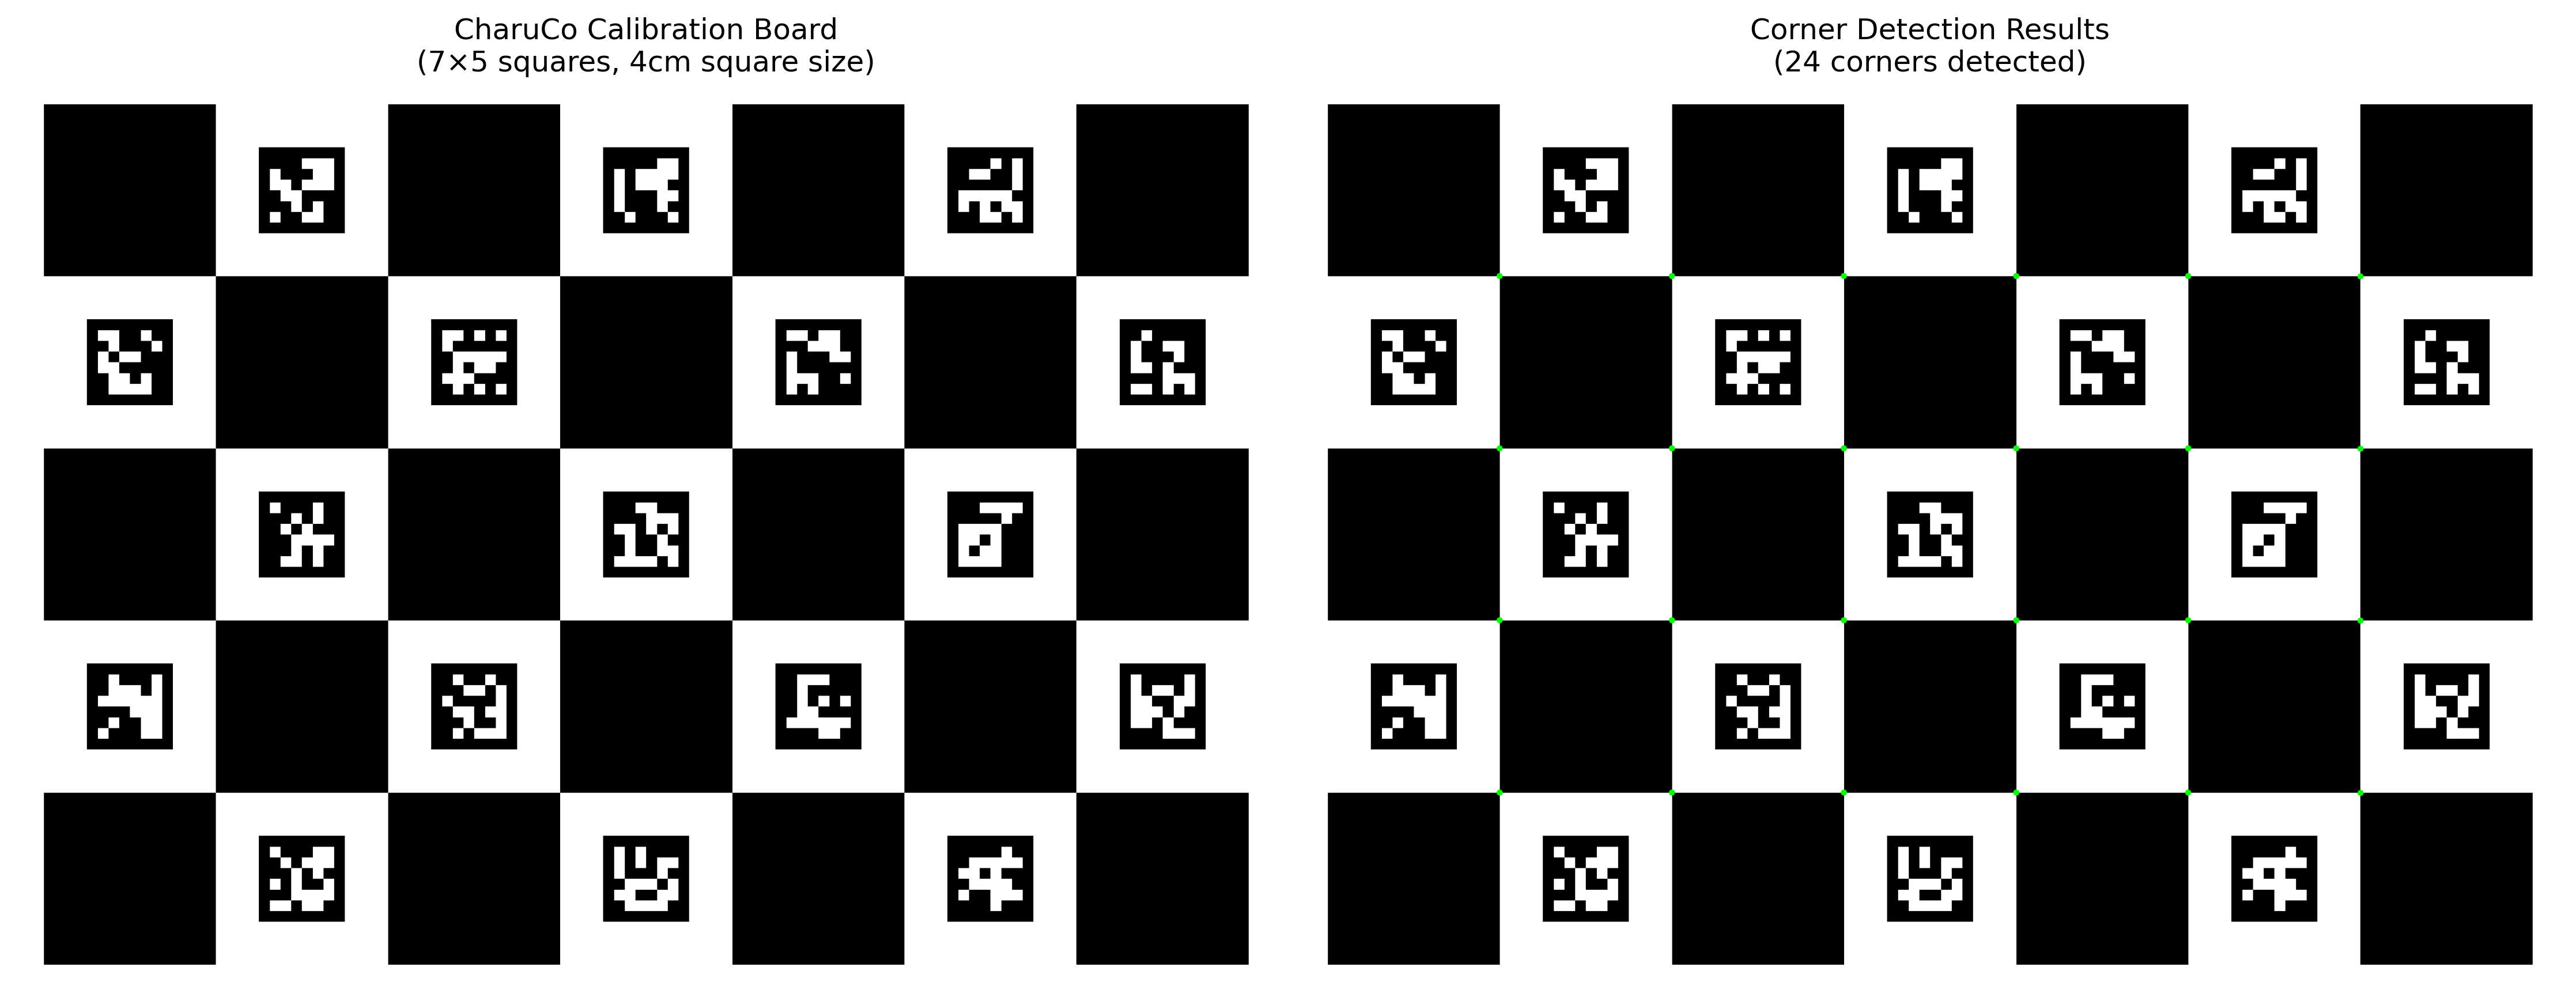
\includegraphics[width=\linewidth]{calibration/charuco_detection_demo.png}
\caption{CharuCo Board \& Detection}
\end{figure}
\end{column}

\begin{column}{0.33\textwidth}
\textbf{Disparity Processing:}
\begin{figure}
\centering
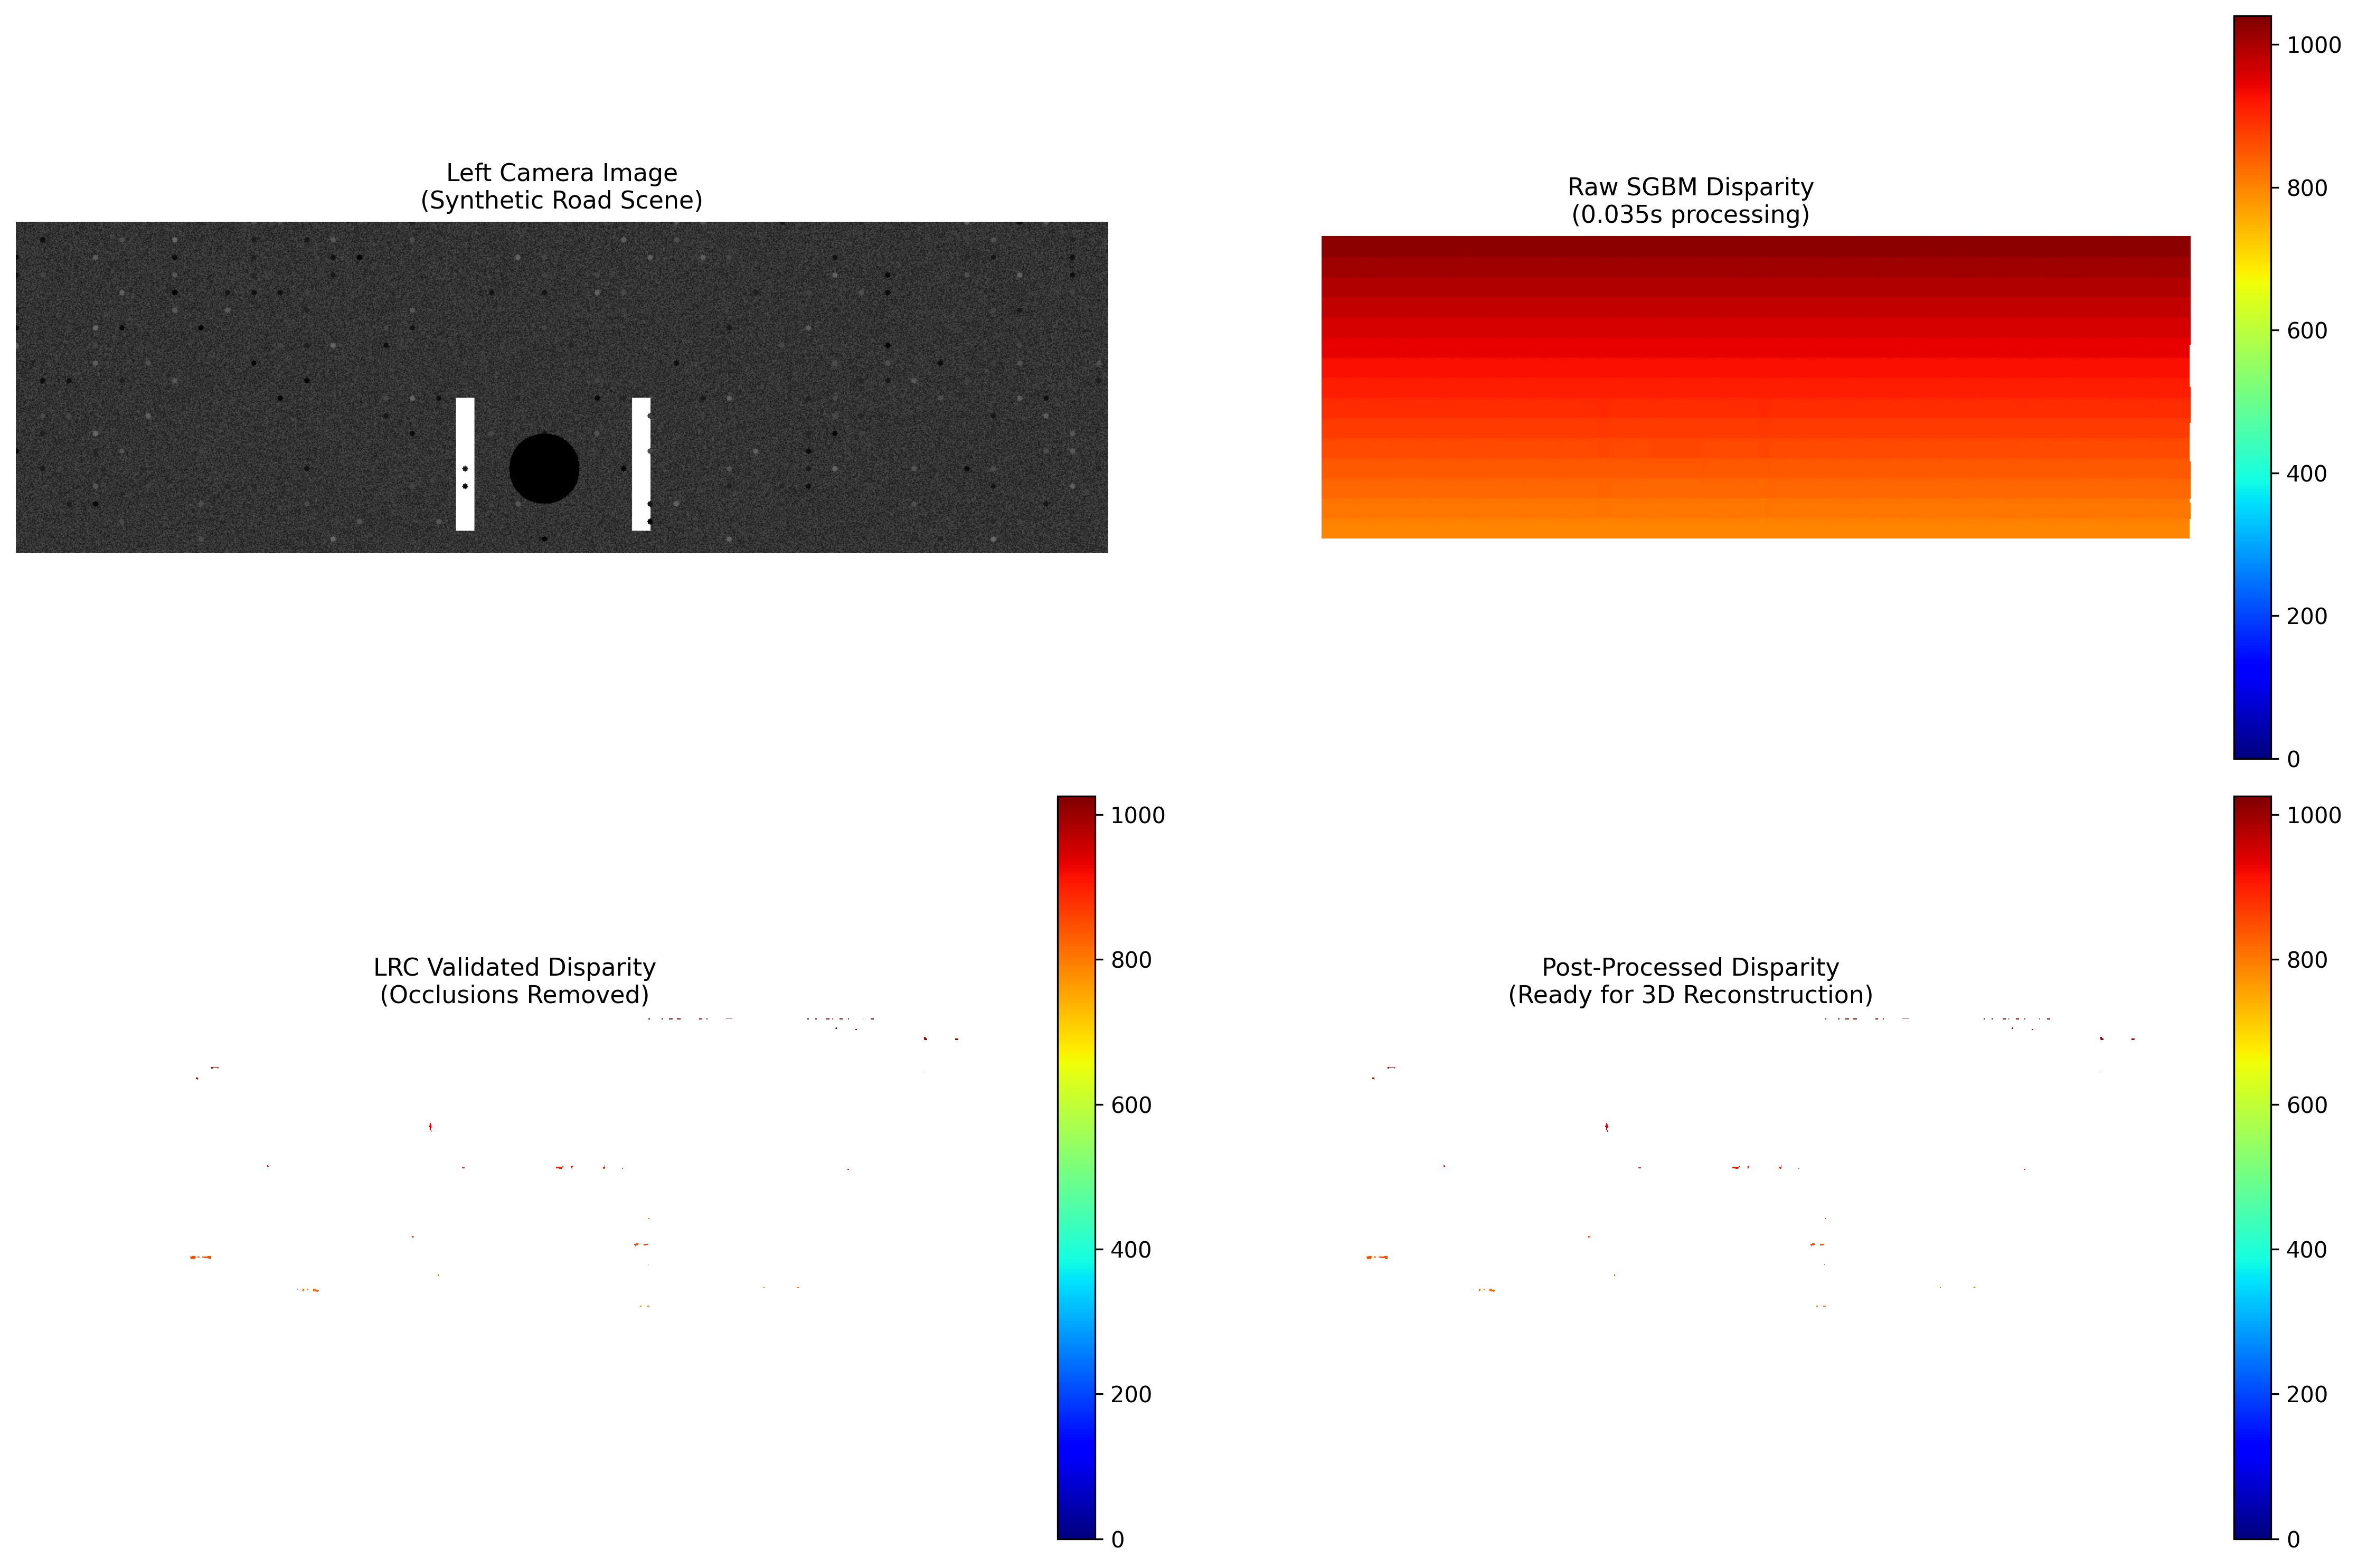
\includegraphics[width=\linewidth]{disparity/disparity_processing_pipeline.png}
\caption{Disparity Pipeline Output}
\end{figure}
\end{column}

\begin{column}{0.33\textwidth}
\textbf{3D Reconstruction:}
\begin{figure}
\centering
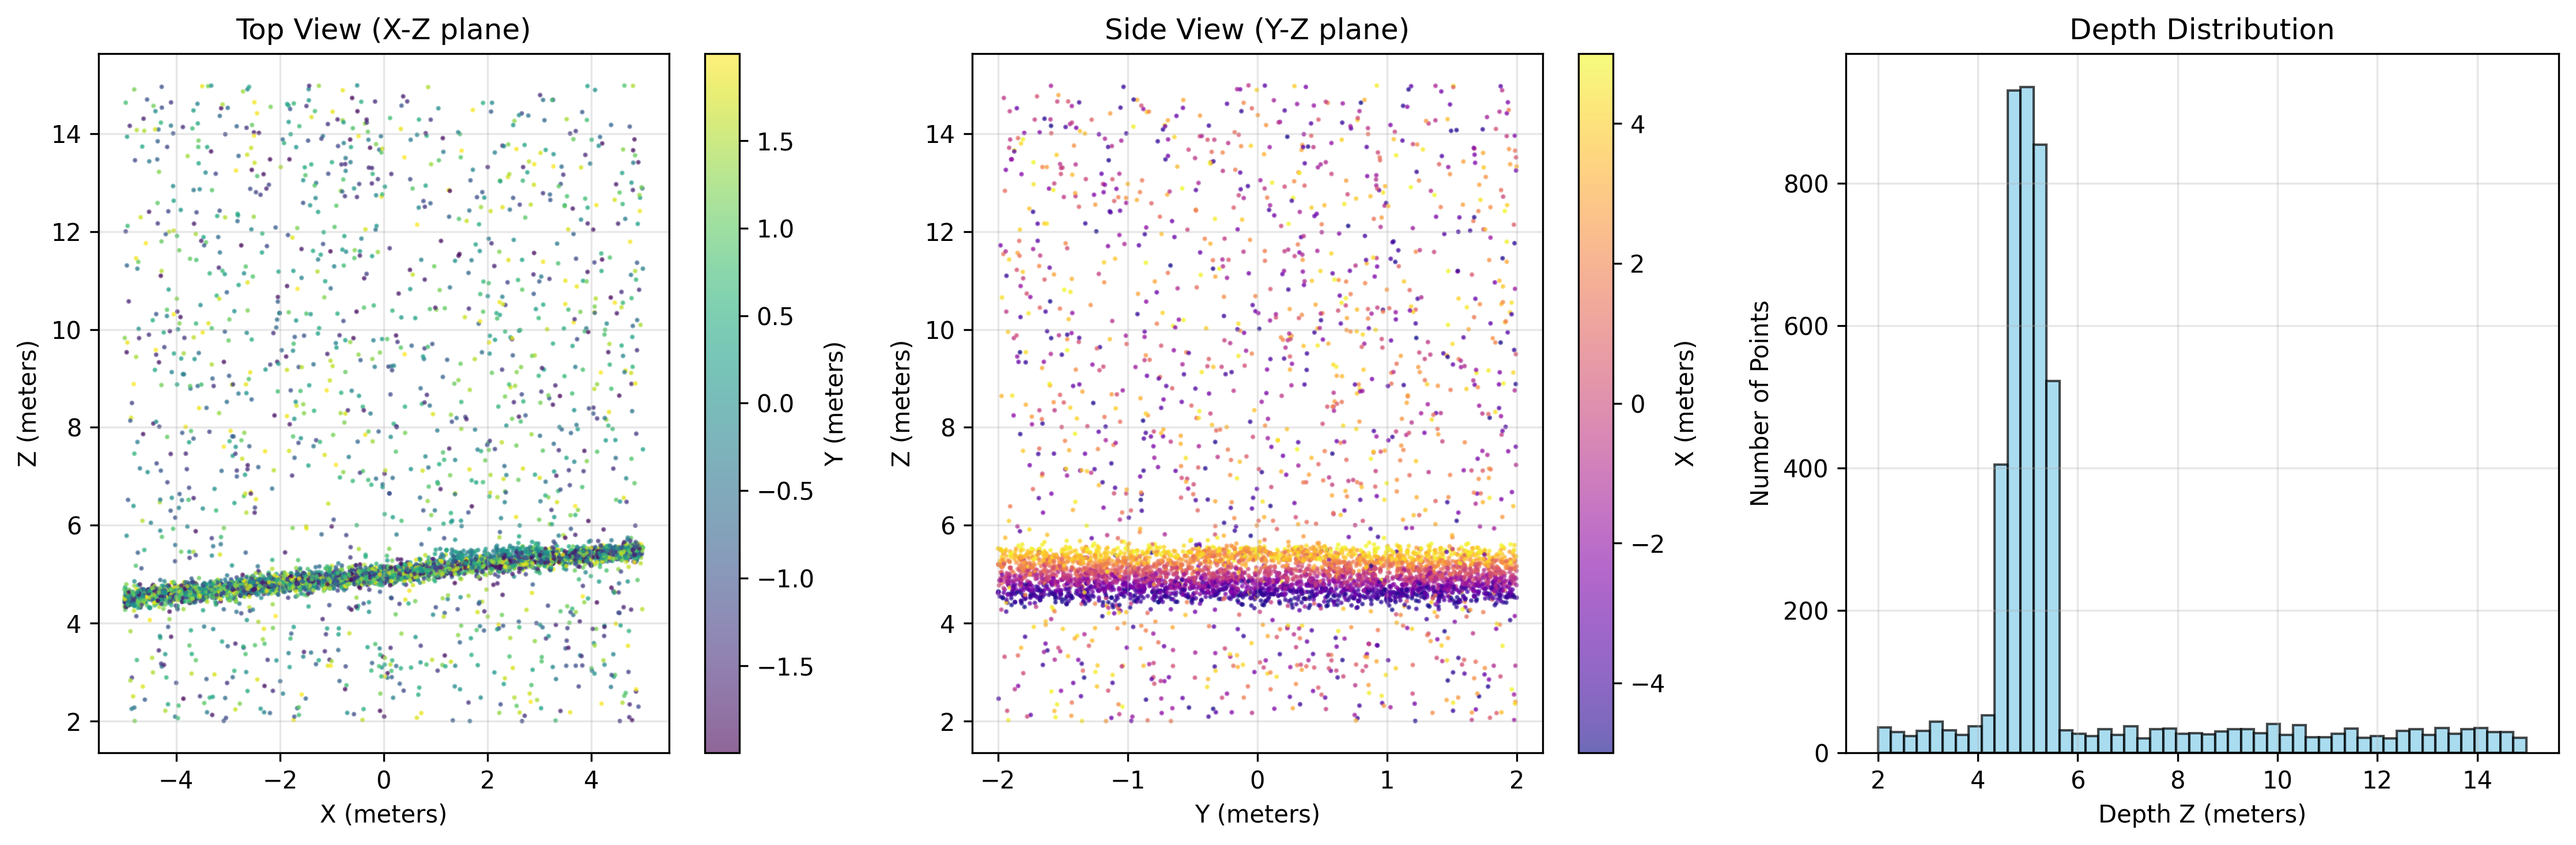
\includegraphics[width=\linewidth]{3d_reconstruction/3d_point_cloud_analysis.png}
\caption{Point Cloud Analysis}
\end{figure}
\end{column}

\end{columns}
\end{frame}

\end{document}






